\documentclass[utf8,10pt]{beamer}

\usepackage{listings}


\usepackage{multirow}
\usepackage{amsmath}
\usepackage{epsfig}
\usepackage{graphicx}
\usepackage{epstopdf}
\usepackage{chemfig}
\usepackage{soul}
\usepackage[dvipsnames]{xcolor}
\usepackage{xcolor}
\usepackage{adjustbox}

\usepackage{CJKutf8}

\lstdefinestyle{shell}{
  language=bash,
  basicstyle=\ttfamily\small,
  keywordstyle=\color{blue!70!black},
  commentstyle=\color{gray}\itshape,
  stringstyle=\color{green!50!black},
  backgroundcolor=\color{gray!8},
  frame=single,
  framesep=4pt,
  rulecolor=\color{gray!40},
  breaklines=true,
  breakatwhitespace=true,
  showstringspaces=false,
  columns=flexible,
}
\lstset{style=shell}

\definecolor{orange}{RGB}{204,0,102}
\definecolor{purple}{RGB}{97,0,255}

\title{The $P_{c}(4337)$ pentaquark \\
  from the $B_s^0 \to J/\psi p \bar{p}$ decays}

\vspace{0.45cm}

\institute{A tutorial for theoreticians}

\begin{document}
\begin{frame}
\titlepage

\vspace{-0.5cm}


\vspace{0.45cm}


\begin{center}
  {\normalsize by Manuel Pavon Valderrama}
\end{center}


\end{frame}
{
%\setbeamercolor{background canvas}{bg=}

}
%---------------------------------------------------------------------- SLIDE -
\begin{frame}
\frametitle{Where has the $P_{c}(4337)$ been seen?}

\vspace{-0.25cm}
\begin{itemize}
\item Observed in the $B_s^0 \to J/\Psi p \bar{p}$ decay:

\vspace{-0.25cm}
\begin{center}
\colorbox{white}{
{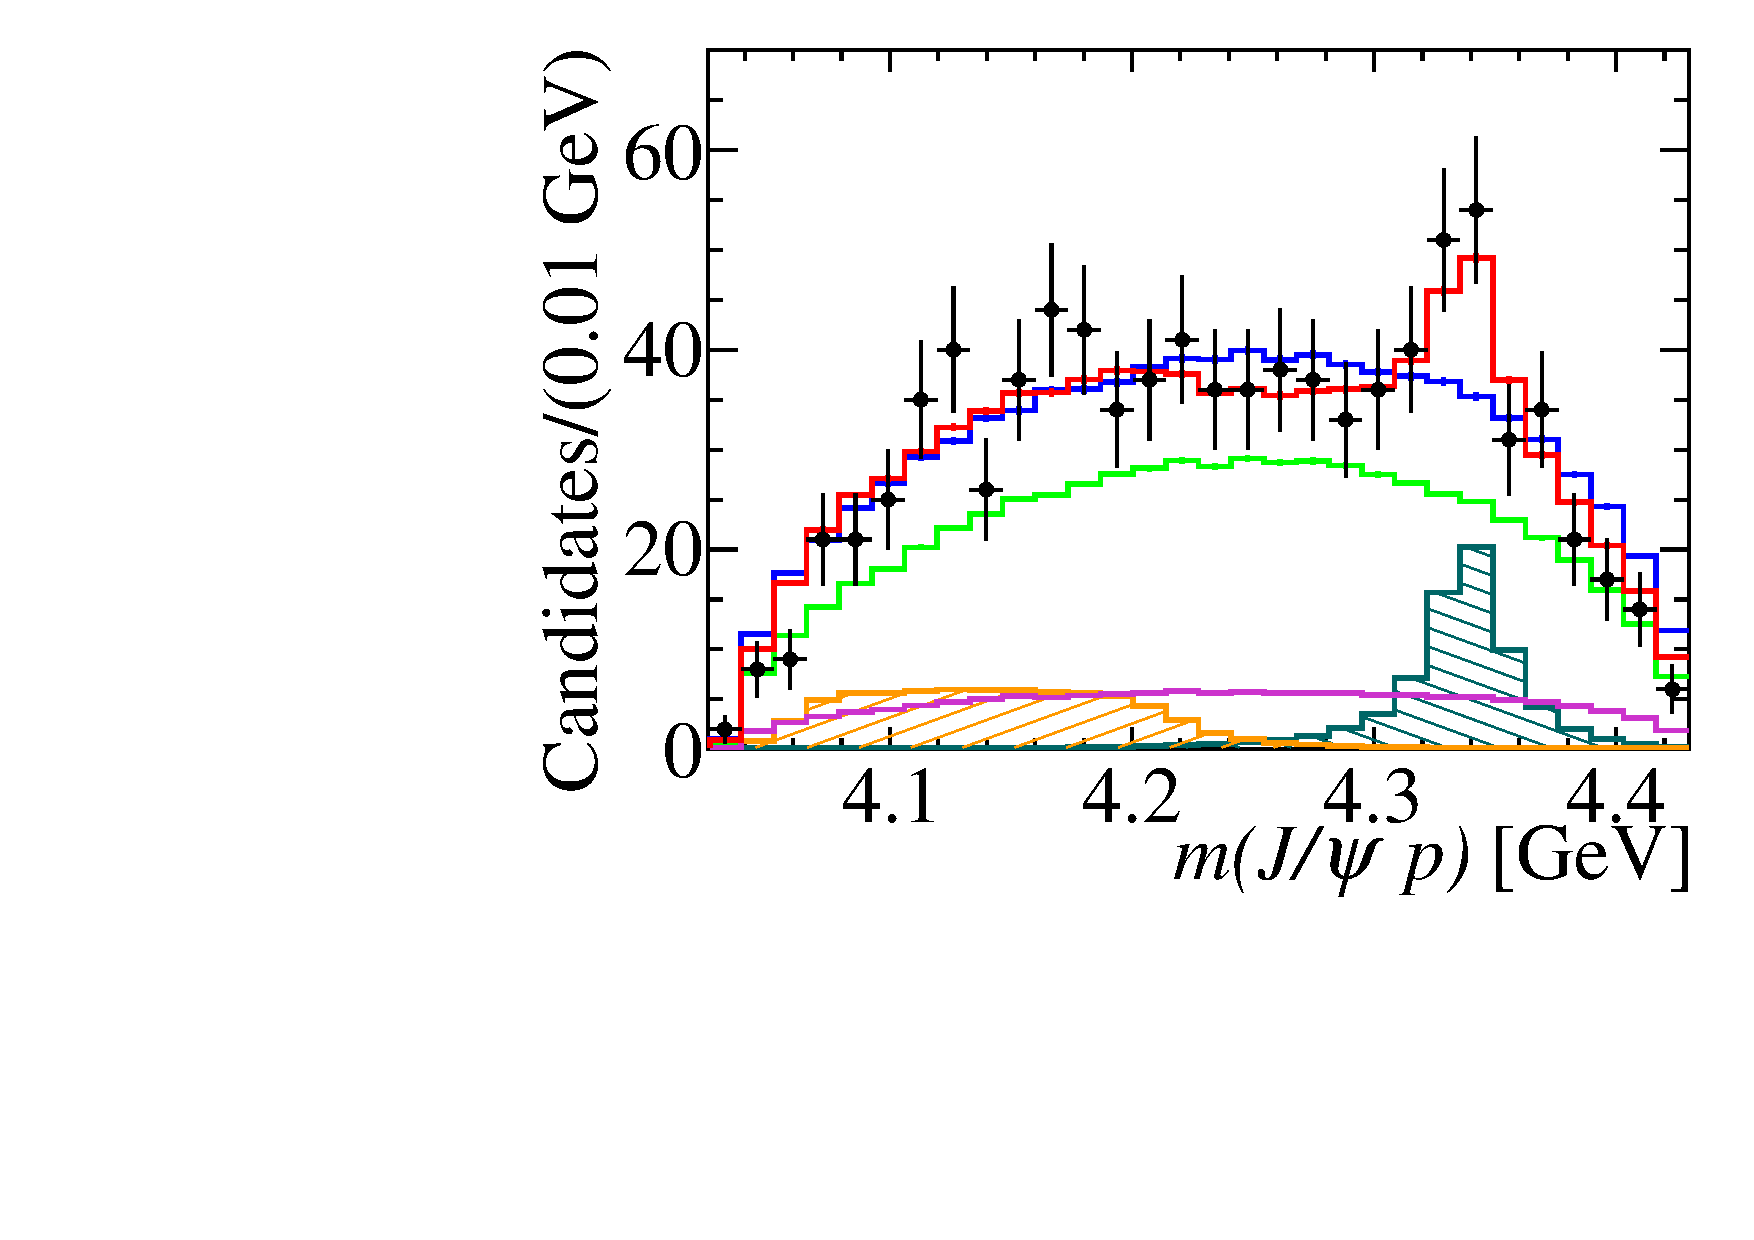
\includegraphics[height=3.5cm]{figures/Pc4337/Fig2e.pdf}}
{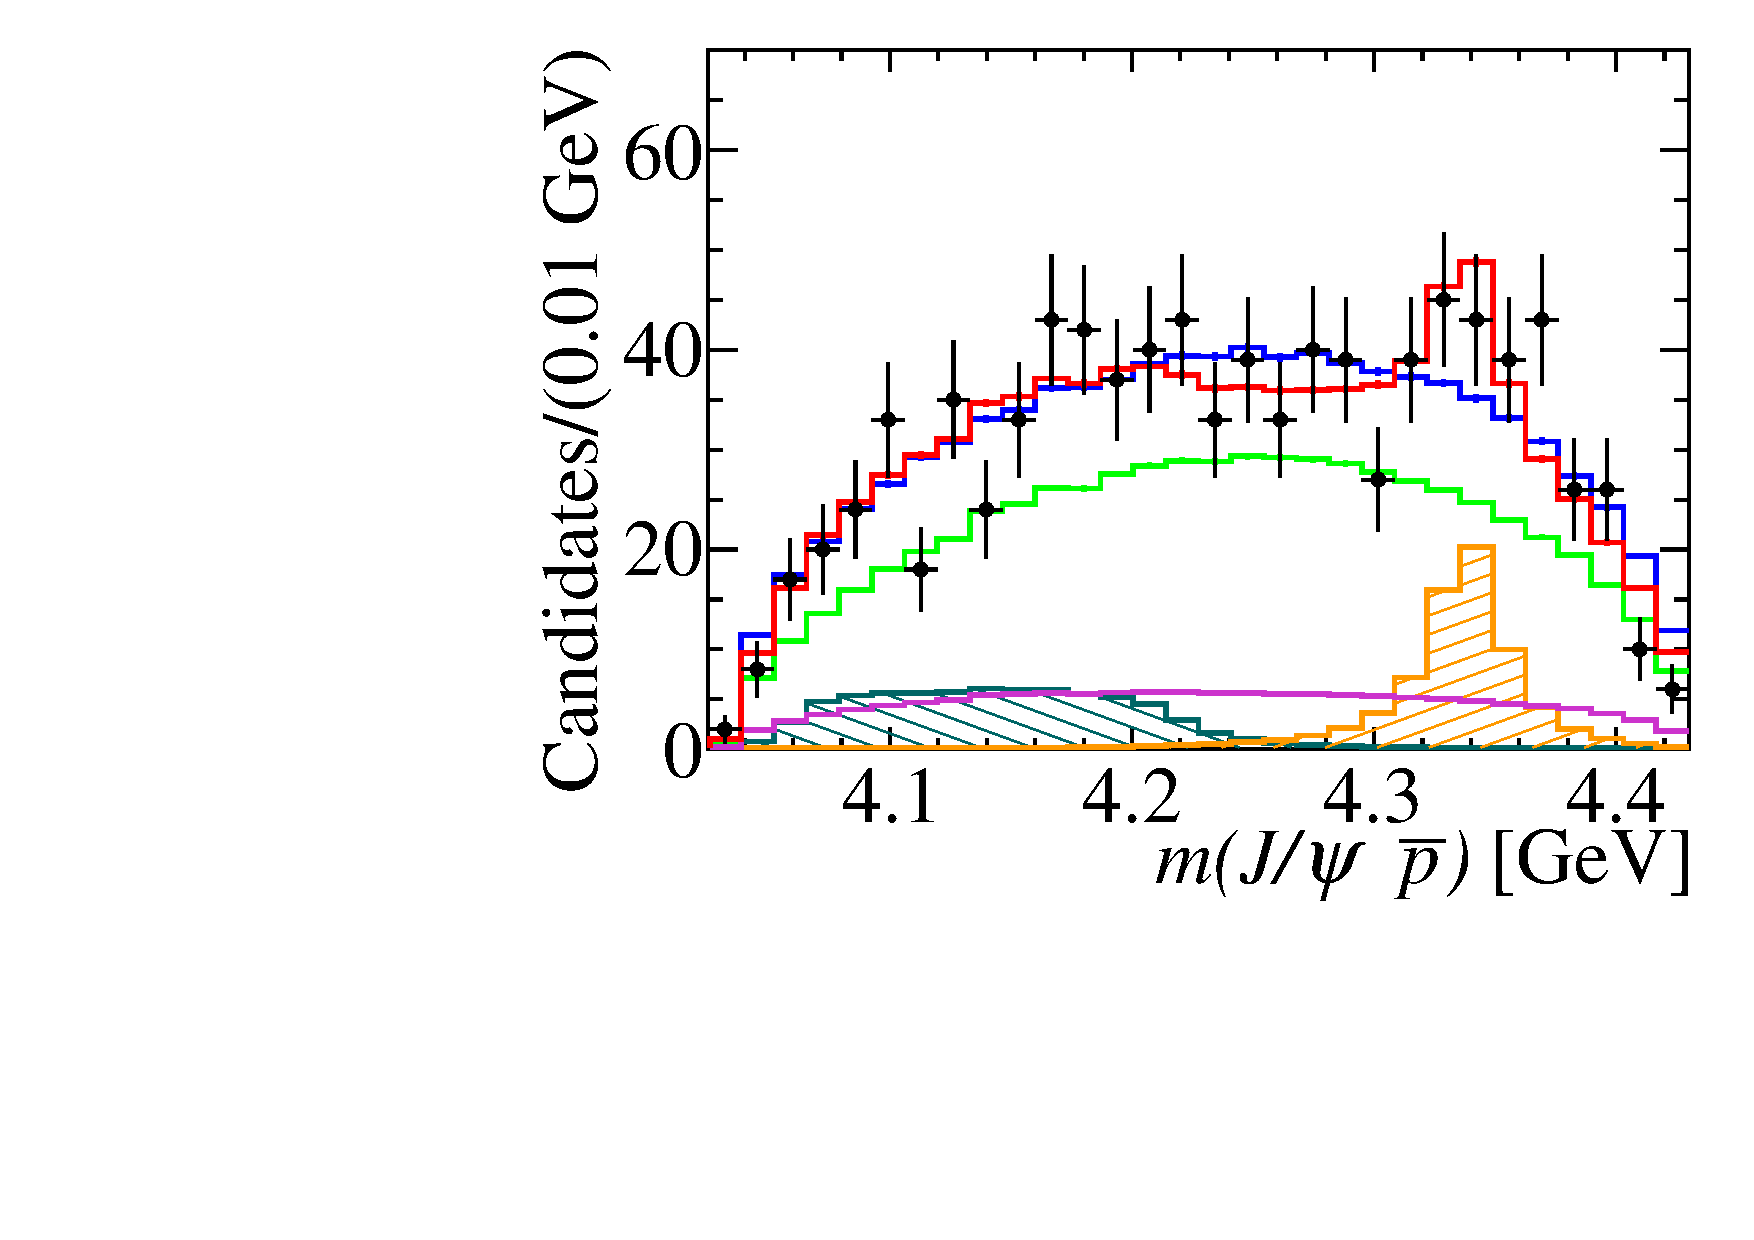
\includegraphics[height=3.5cm]{figures/Pc4337/Fig2f.pdf}}
}
\end{center}

\item $J^P = \frac{1}{2}^+$, $\frac{1}{2}^-$ (preferred choices)  

\item $M = 4337^{+7}_{-4} {}^{+2}_{-2}\,{\rm MeV}$, $\Gamma = 29^{+26}_{-12} {}^{+14}_{-14}\,{\rm MeV}$ \\
  (for $\frac{1}{2}^+$, slightly different for $\frac{1}{2}^-$)

\item Statistical significance not strong ($3.7\,\sigma$ for $\frac{1}{2}^+$, $3.5\,\sigma$ for $\frac{1}{2}^-$) 
\end{itemize}

\end{frame}
%---------------------------------------------------------------------- SLIDE -
\begin{frame}
\frametitle{$P_{c}(4337)$ pentaquark: the invariant mass (Ia)}

A bird's eye view of how this works (a): 

\begin{itemize}
\item[(i)] We write down the diagrams:

\vspace{-0.15cm}
\begin{center}
\colorbox{white}{
    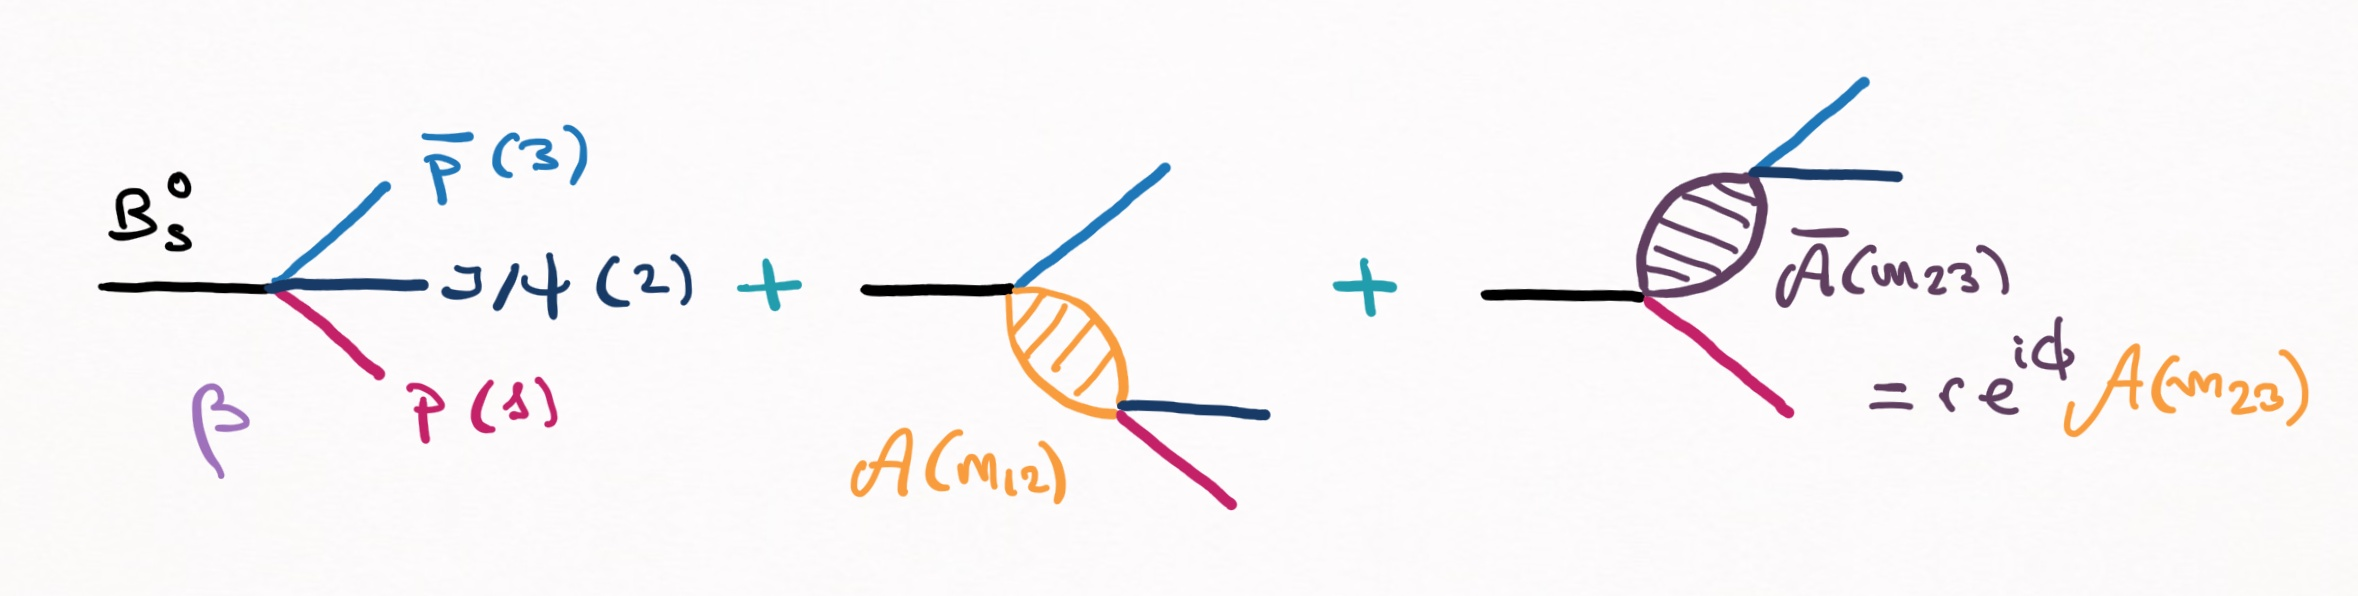
\includegraphics[height=2.24cm]{figures/Pc4337/diagrams-Bs0-decay.jpeg}
}
\end{center}

where $\beta$ is the non-resonant amplitude and $\mathcal{A}$ the pentaquark
amplitude. For simplicity, $r\, e^{i \phi} = +1$ for $J^P = \frac{1}{2}^-$ {\color{magenta} ${}^{(*)}$}.

\item[(ii)] The invariant mass distribution reads {\color{magenta} ${}^{(**)}$} (scalar approximation):

\vspace{-0.25cm}
{\small $$
\frac{d\Gamma}{d m_{12}} \propto m_{12}\,\int_{{(m_{23})}^2_{\rm min}}^{{(m_{23})}^2_{\rm max}}
{\Big| \beta +  \underbrace{\mathcal{A}(m_{12})}_{\rm main\,\,peak(s)} + \underbrace{r\,e^{i \phi} \mathcal{A}(m_{23})}_{\rm reflection(s)} \Big|}^2\,d m_{23}^2
$$}

\vspace{-0.15cm}
where spin factorizes in the non-relativistic limit for $J^P = \frac{1}{2}^-$.

\end{itemize}

{\scriptsize {\color{magenta} $(*)$} Per appendix A of arXiv:2108.04720, between Eqs. (22) and (23). \\
  {\color{magenta} $(**)$} Check the PDG review on kinematics }

\end{frame}
%---------------------------------------------------------------------- SLIDE -
\begin{frame}
\frametitle{$P_{c}(4337)$ pentaquark: the invariant mass (Ib)}

A bird's eye view of how this works (b): 

\begin{itemize}
\item[(iii)] The observed invariant mass distribution is in counts per bin:

\vspace{-0.15cm}
\begin{center}
\colorbox{white}{
{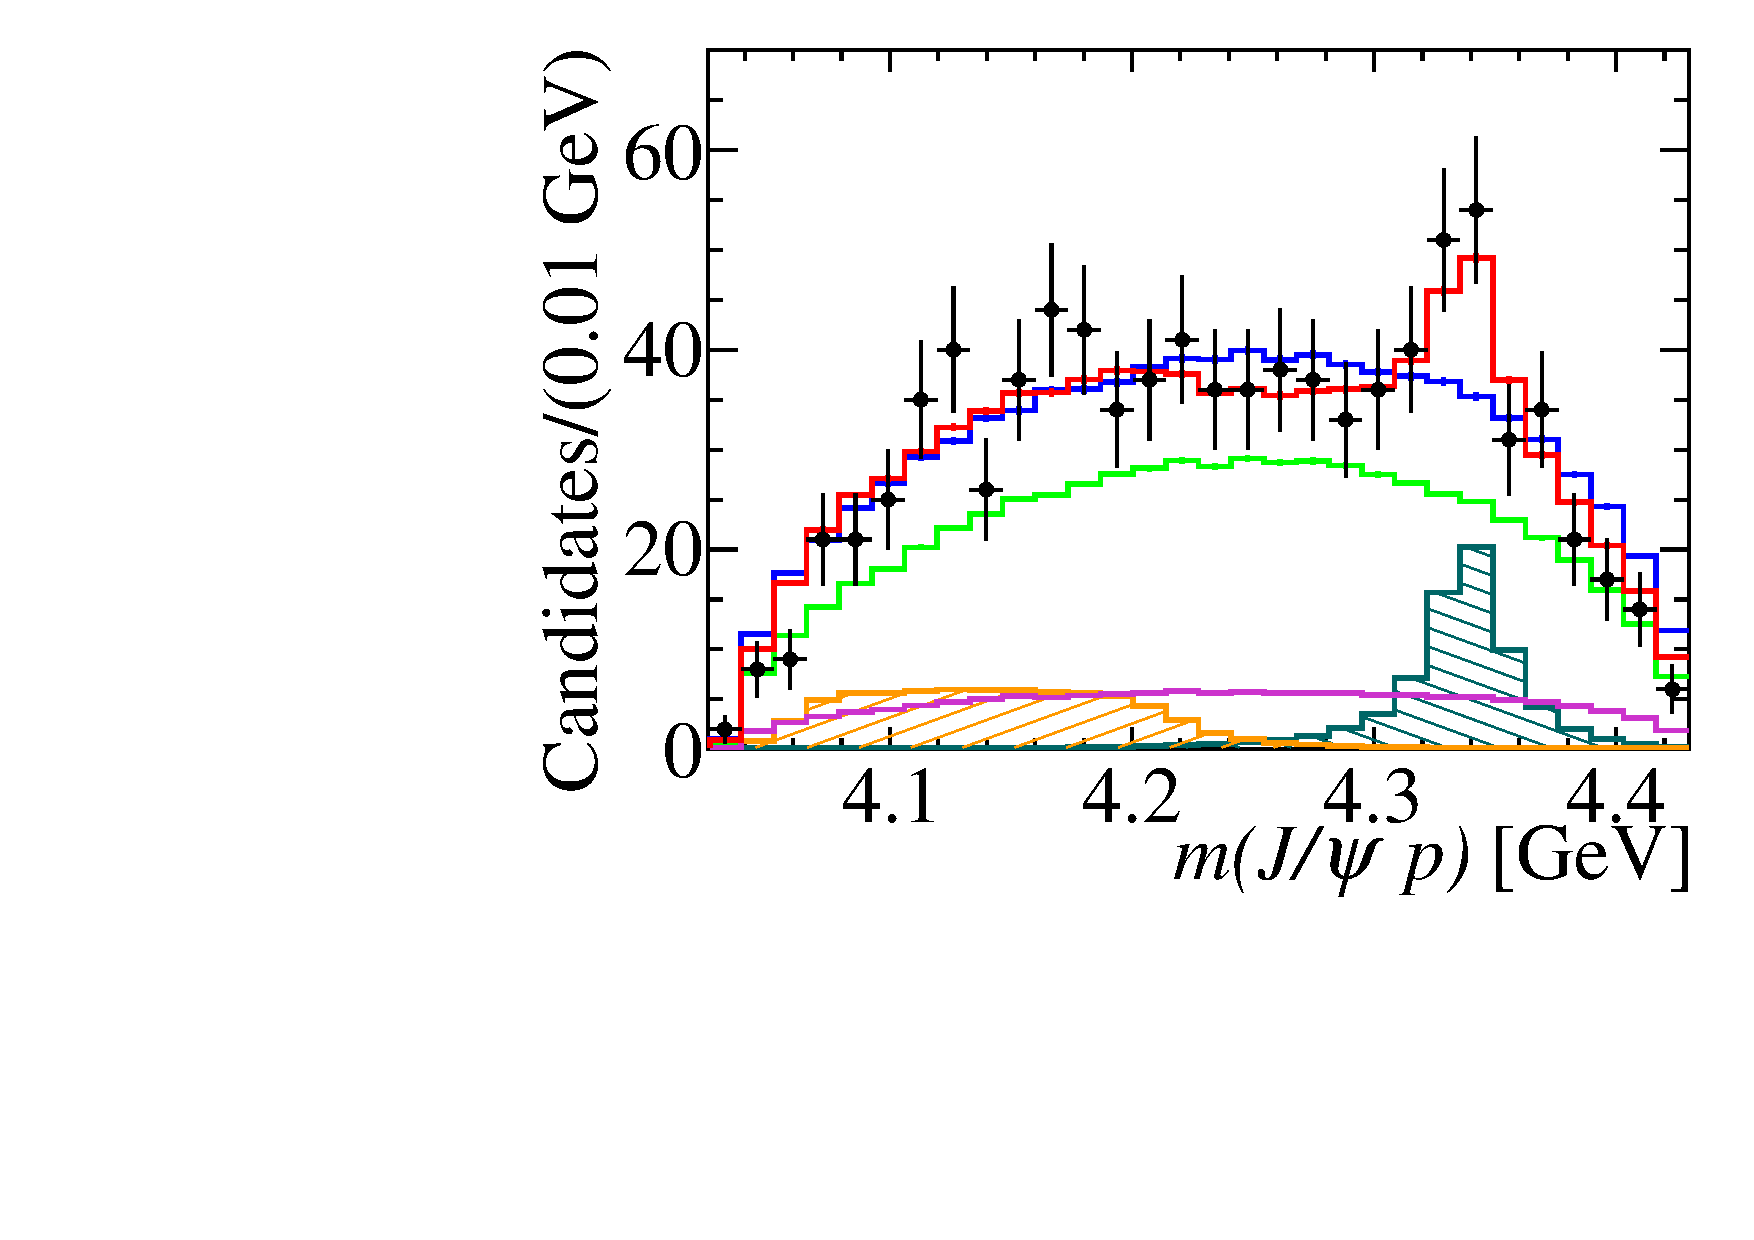
\includegraphics[height=3.2cm]{figures/Pc4337/Fig2e.pdf}}
{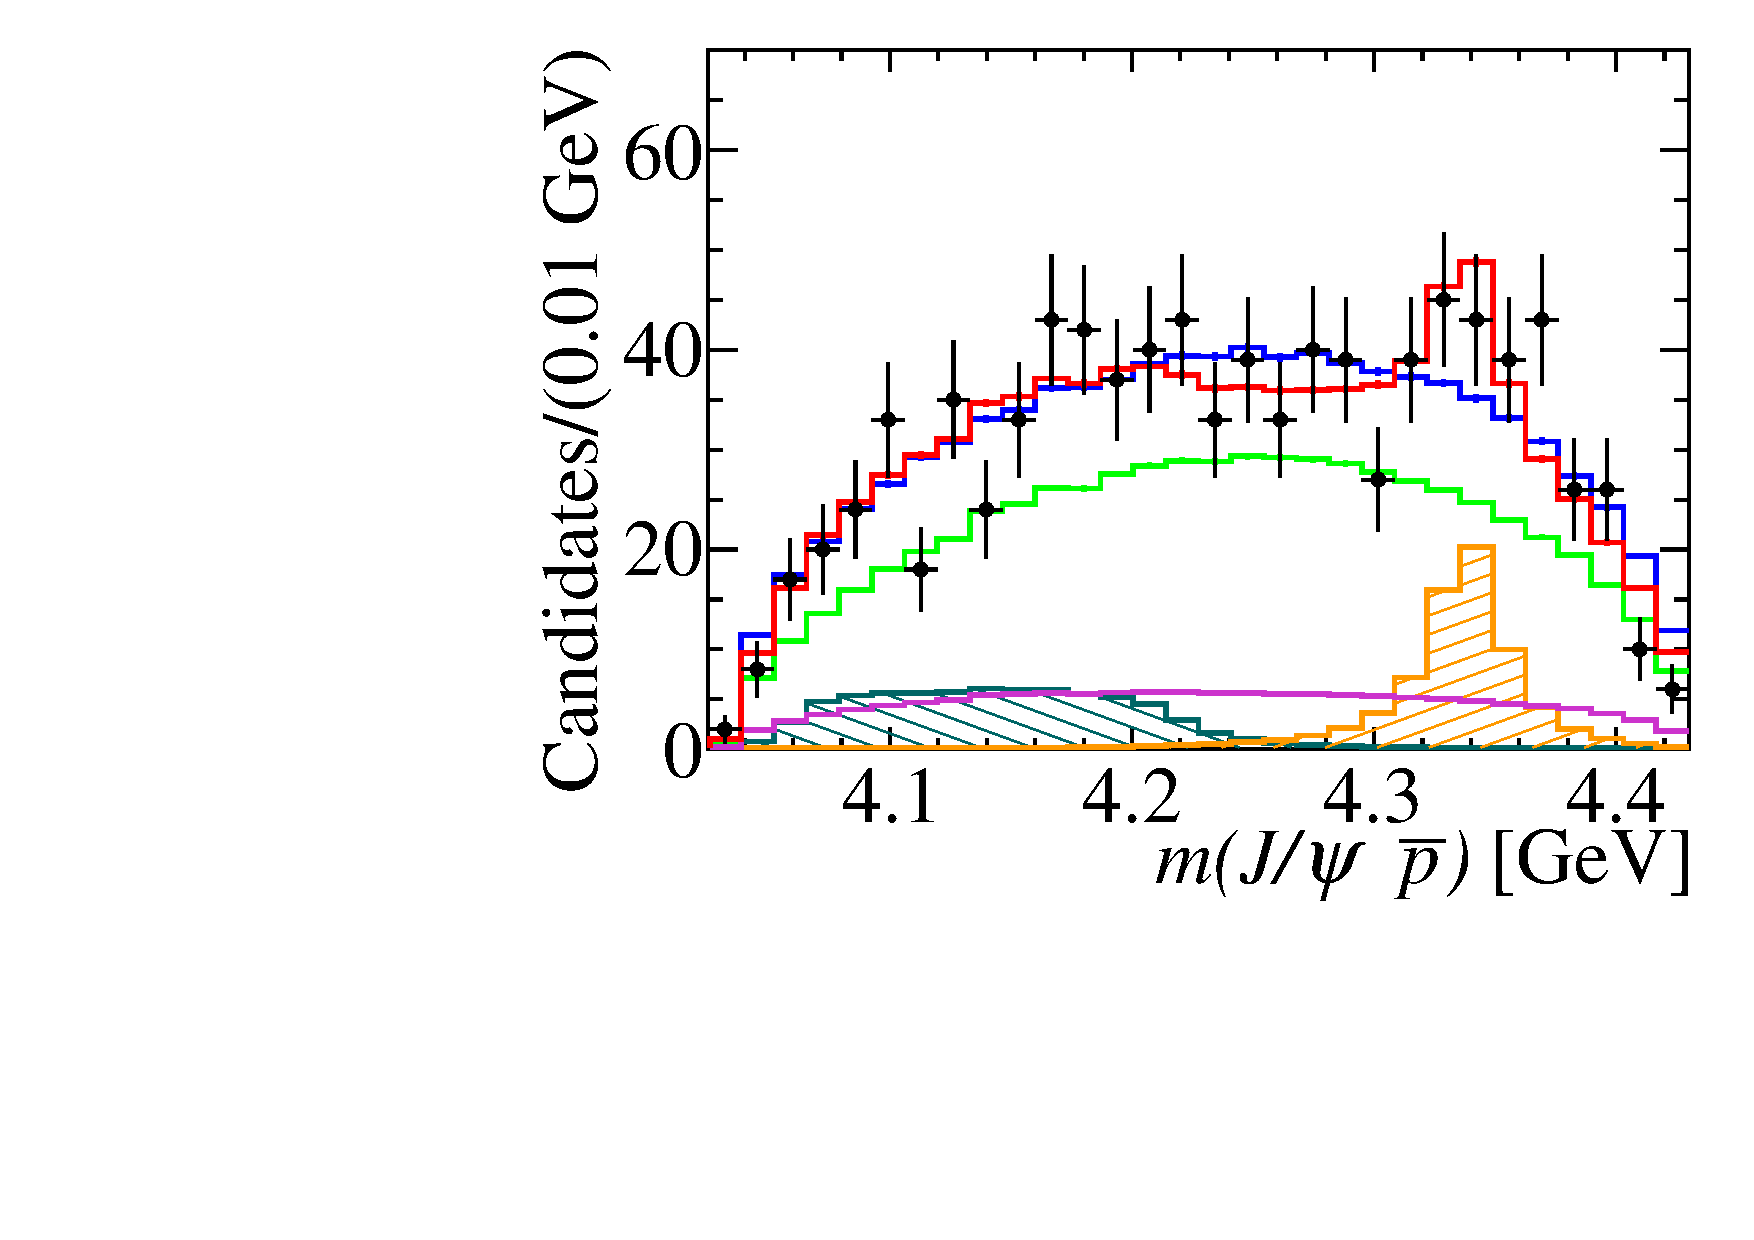
\includegraphics[height=3.2cm]{figures/Pc4337/Fig2f.pdf}}
}
\end{center}

\item[(iv)] The theoretical counts are proportional to the sum of $d\Gamma/dm_{12}$ over bin $i$, to which one adds the expected counts of
  the incoherent background $B_i$:

  \vspace{-0.25cm}
  {\small
  $$
    N_i^{\rm th} = B_i + \mathcal{N}\,\int_{(m_{12})_{\rm min}}^{(m_{12})_{\rm max}} \,
    \frac{d \Gamma}{d m_{12}}\, d m_{12} \, ,
  $$}

  the bin limits, size ($13.5\,{\rm MeV}$), counts and background can be
  extracted from the $*.C$ files in the preprint source.
  
\end{itemize}

\end{frame}
%---------------------------------------------------------------------- SLIDE -
\begin{frame}
\frametitle{$P_{c}(4337)$ pentaquak: the invariant mass (Ic)}

A bird's eye view of how this works (c): 

\begin{itemize}
\item[(v)] The number of events per bin follows a Poisson distribution (derived from the individual probabilities for each bin). \\
  \vspace{0.15cm}
  Thus one fits to the bin counds by minimizing {\color{magenta} ${}^{(*)}$ }

  {\small
    $$
    D = \sum_i 2\left( N_i^{\rm th} - N_i^{\rm exp} + N_i^{\rm exp} \log{\frac{N_i^{\rm exp}}{N_i^{\rm th}}} \right)
    $$
  }

  except if $N_i^{\rm th} = 0$, in which case one simply adds $2 N_i^{\rm th}$.
  
\item[(vi)] However, the invariant mass distributions contain much less
  information   than the 4-dimensional fit from the LHCb, which includes
  the decay into muons, i.e. $B_s^0 \to J/\psi (\to \mu^+ \mu^-) p \bar{p}$,
  depending on the variables $m_{p\bar{p}}$, $\theta_p$, $\theta_{\mu}$,
  $\varphi$ {\color{magenta} ${}^{(**)}$ }.
\end{itemize}

{\scriptsize {\color{magenta} $(*)$} Check the PDG review on statistics.\\
  {\color{magenta} $(**)$} Check the LHCb paper for details}
\end{frame}
%---------------------------------------------------------------------- SLIDE -
\begin{frame}
\frametitle{$P_{c}(4337)$ pentaquak: the invariant mass (Id)}

A bird's eye view of how this works (d): 

\begin{itemize}
  \item[(vii)] The different mass distributions are correlated: the previous
    minimization for Poisson distributions only makes statistical sense
    for events that are independent from each other. \\
    \vspace{0.15cm}
    That is, the minimum of $D$ only has a clear statistical significance
    when applied to one of the three mass distributions, either
    $M(J/\psi p)$, $M(J/\psi \bar{p})$ or $M(p \bar{p})$. \\
    \vspace{0.15cm}
    This should be taken into account if one decides to fit two or more of
    them at the same time.
    
  \item[(viii)] A better setup to avoid the aforementioned correlations would
    be to fit instead to the event count of the binned Dalitz plot.
    They directly proportional to the integral of
    $|\beta + \mathcal{A}_{12} + \mathcal{A}_{23}|^2$ in the square bin. \\
    \vspace{0.15cm}
    The $*.C$ file for the Dalitz plot is \texttt{Fig2.C} (which is not
    immediately clear from the manuscript, as the Dalitz plot is Fig.3)!
\end{itemize}

\end{frame}
%---------------------------------------------------------------------- SLIDE -
\begin{frame}
\frametitle{$P_{c}(4337)$ as a Breit-Wigner (I)}

The easiest parametrization is to consider a Breit-Wigner (BW), which for $J^P = \frac{1}{2}^-$ (or, better said, $L = 0$) gives the amplitude:

{$$
  \mathcal{A}(m) = \frac{g}{M^2 - m^2 - i M\,\Gamma(m)} \quad \mbox{with} \quad
  \Gamma(q) = \frac{q(m)}{q(M)} \frac{M}{m}\,\Gamma
  $$}

with $M$, $\Gamma$ the mass and width of the resonance and $g$ complex; $q(m)$
is defined either in the LHCb manuscript or in the programs.

\vspace{0.25cm}
The BW fit can be compiled with and run with:

\hspace{0.5cm} \texttt{\$ make imd\_bw}  \\
\hspace{0.5cm} \texttt{\$ ./imd\_bw} 

by default it fits to $M(J/\psi p)$, which yields:
\begin{itemize}
\item $M = 4340\,{\rm MeV}$, $\Gamma = 29\,{\rm MeV}$, which looks sensible,
\end{itemize}
and has $D = 18.7$ or $D/(N_{\rm bins} - N_{\rm params}) \sim 0.75$, which is good.

\end{frame}
%---------------------------------------------------------------------- SLIDE -
\begin{frame}
\frametitle{$P_{c}(4337)$ as a Breit-Wigner (II)}

The obtained $M(J/\psi p(\bar{p}))$ and $\cos{\theta_p}$ distributions are (histograms):

\vspace{-0.15cm}
\begin{center}
\colorbox{white}{
{\includegraphics[height=4.0cm]{gnuplot/M12-fit12-BW-bins.eps }}
{\includegraphics[height=4.0cm]{gnuplot/Mz-fit12-BW-bins.eps }}
}
\end{center}

But there is a problem that highlights that we have less information
than in the LHCb fit...


\end{frame}
%---------------------------------------------------------------------- SLIDE -
\begin{frame}
\frametitle{$P_{c}(4337)$ as a Breit-Wigner (III)}

If I fit instead to $M(J/\psi \bar{p})$, the resonance becomes {\color{red} too broad}
\begin{itemize}
  \item $M = 4378\,{\rm MeV}$, $\Gamma = 89\,{\rm MeV}$ {\color{red} (!)},
\end{itemize}
with $D = 26.0$, which is still good. The distributions are now:

\vspace{-0.15cm}
\begin{center}
\colorbox{white}{
{\includegraphics[height=4.0cm]{gnuplot/M12-fit23-BW-bins.eps }}
{\includegraphics[height=4.0cm]{gnuplot/Mz-fit23-BW-bins.eps }}
}
\end{center}

The reasons are that (i) the non-resonant amplitude is not flat,
(ii) detector efficiency effects and (iii) the distributions are
projections of the more information rich phase space of
$B_s^0 \to J/\psi(\to \mu^+ \mu^-) p \bar{p}$. 


\end{frame}
%---------------------------------------------------------------------- SLIDE -
\begin{frame}
\frametitle{$P_{c}(4337)$ as a Breit-Wigner (IV)}

We may fit to more than one of the distributions, though
this ignores the existence of statistical correlations among them:

\begin{itemize}
\item[(i)] By fitting to $M(J/\psi p)$ and $\cos{\theta_p}$ distros: \\
  \begin{itemize}
  \item  $M = 4350\,{\rm MeV}$, $\Gamma = 53\,{\rm MeV}$
   \end{itemize}
  with $D = 41.8$, or $D/(N_{\rm bins} - N_{\rm params}) \sim 0.76$
\item[(ii)] By fitting to $M(J/\psi p)$, $M(J/\psi \bar{p})$ and $\cos{\theta_p}$ distros:
  \begin{itemize}
  \item  $M = 4362\,{\rm MeV}$, $\Gamma = 79\,{\rm MeV}$
  \end{itemize}
    with $D = 75.8$, or $D/(N_{\rm bins} - N_{\rm params}) \sim 0.89$
\end{itemize}

{\color{magenta} {\bf caveat}: the statistical interpretation of the Poisson deviation is unclear} \\

\vspace{0.2cm}
       {(because of unaccounted correlations among the distros,
         the most obvious example being the $M(J/\psi p)$ and
         $M(J/\psi \bar{p})$ distros)}

\end{frame}
%---------------------------------------------------------------------- SLIDE -
\begin{frame}
\frametitle{$P_{c}(4337)$ as a Breit-Wigner (V)}

A different possibility is to fit directly to the binned Dalitz plot.

\vspace{0.15cm}

This Fig. 3 in the LHCb manuscript: the binned Dalitz plot uses a
18 x 18 square grid, where 149 bins contain part of the
kinematically allowed regions; 136 bins have at least 1 count.

\vspace{0.15cm}

The fit yields:
\begin{itemize}
  \item $M = 4374\,{\rm MeV}$, $\Gamma = 128\,{\rm MeV}$
\end{itemize}
    with $D = 136.0$, or $D/(N_{\rm bins} - N_{\rm params}) \sim 0.94$



\end{frame}
%---------------------------------------------------------------------- SLIDE -
\begin{frame}
\frametitle{$P_{c}(4337)$ as a Breit-Wigner (VI)}

Thus the best option is to improve the non-resonant amplitude:

\vspace{0.15cm}

{\color{red} Right now this is work in progress}

\end{frame}
%---------------------------------------------------------------------- SLIDE -
\begin{frame}
\frametitle{$P_{c}(4337)$ as a meson-baryon molecule (I)}

\vspace{-0.35cm}

For a meson-baryon loop with rescattering the relevant diagram is:

\vspace{-0.15cm}
\begin{center}
\colorbox{white}{
    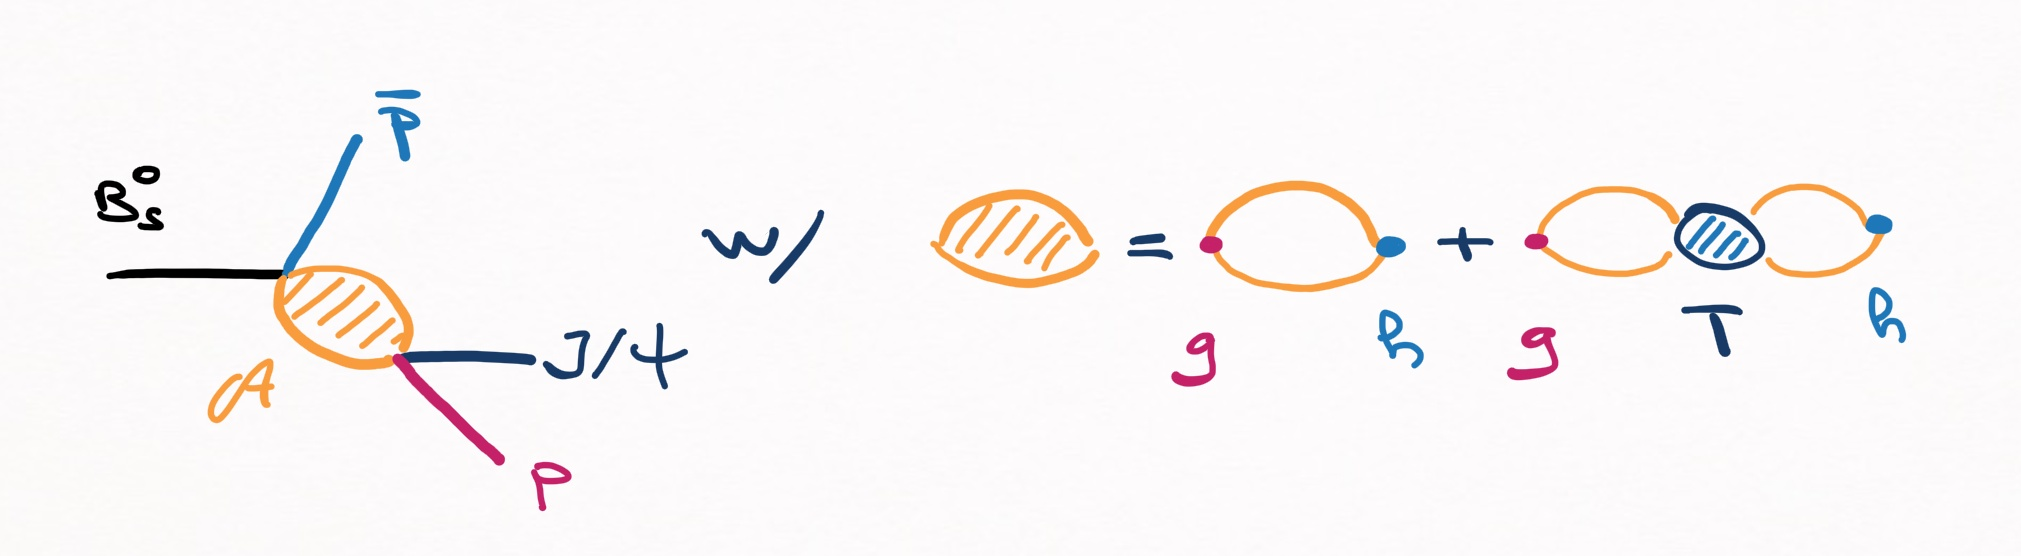
\includegraphics[height=2.24cm]{figures/Pc4337/Diagrams-meson-baryon-rescattering.jpeg}
}
\end{center}

which leads to the amplitude

\vspace{-0.15cm}
{$$
\mathcal{A}(m) = g\,\left( G_0 + G_0 T(E) G_0 \right)\,h \, ,
$$}

where $g$ and $h$ are the production/decay couplings,
$G_0 = G_0(E)$ the loop function
and $T(E)$ the T-matrix, with $E = m - m_{\rm th}$ (and $m_{\rm th}$ the mass
of the meson-baryon threshold)

\vspace{0.25cm}

A more detailed explanation follows in the next slides...

\end{frame}
%---------------------------------------------------------------------- SLIDE -
\begin{frame}
\frametitle{$P_{c}(4337)$ as a meson-baryon molecule (II)}

\vspace{-0.35cm}

\begin{itemize}
\item In general $g$ is complex and $h$ real and only their product matters. \\
  One can set $h=1$ (if there are no coupled channels). \\
  \vspace{0.15cm}
         {\scriptsize {\color{magenta} Caveat:} $h$ contributes to the decay
           width or self-energy of the meson-baryon system, \\ but this will be
           ignored in a first approximation}

       \item The loop function reads:

         {\small
         $$
         G_0(E) = \int_{\Lambda} \frac{d^3 \vec{q}}{(2\pi)^2} \frac{1}{m - m_{\rm th} - \frac{q^2}{2\mu} + i \epsilon}
         = \frac{1}{2\pi^2}\,\int_0^{\infty}\,q^2\,dq
         \frac{f^2(q/\Lambda)}{E - \frac{q^2}{2\mu} + i \frac{\Gamma_{\rm th}}{2} + i \epsilon }
         $$}

         which is divergent and requires regularization, where in the
         rightmost term a separable regulator $f(x)$ has been chosen \\
         (more on that later). \\

         \vspace{0.15cm}
         Notice that $m - m_{\rm th} = E + i \Gamma_{\rm th}/2$,
         where $\Gamma_{\rm th}$ here is
         the sum of individual widths of the meson and baryon; $\mu$ is
         the reduced mass and the loop kinematics are non-relativistic
         (heavy hadrons)
\end{itemize}

\end{frame}
%---------------------------------------------------------------------- SLIDE -
\begin{frame}
\frametitle{$P_{c}(4337)$ as a meson-baryon molecule (III)}

\begin{itemize}
\item For the T-matrix one has $T(E) = V + V G_0 T$, where $V$ a contact-range
  potential regularized as

  \vspace{-0.15cm}
  {\small $$
  \langle p' | V | p \rangle = C_0(\Lambda)\,
  f(\frac{p'}{\Lambda}) f(\frac{p}{\Lambda})
  $$}

  in which case

  \vspace{-0.25cm}
  {\small $$
  \langle p' | T(E) | p \rangle = f(\frac{p'}{\Lambda})\,T(E)\,f(\frac{p}{\Lambda}) \quad \mbox{with} \quad   T(E) = {\left[ 1 - C_0 G_0(E) \right]}^{-1}\,C_0
  $$}

\item For a Gaussian regulator $f(x) = e^{-x^2}$, the loop integral reduces to

       {\small
         $$
         G_0(E) = \frac{\mu}{\pi^2}\,\left[ -\sqrt{\pi}{2}\,\Lambda
           + \frac{\pi}{2}\,k\,e^{-2 k^2/\Lambda^2}\,\left( -i +
           {\rm erfi}(\sqrt{2}\frac{k}{\Lambda}) \right)
           \right]
         $$}  

       with ${\rm erfi}$ the imaginary error function
       (${\rm erfi}(z) = {\rm erf}(i z)/i$).
       
     \item Here I have implicitly assumed the $f(x)$ regulator to also appear
       in the production and decay vertices. One can in principle consider
       more phenomenologically motivated regulators/form factors. \\
       {\scriptsize However, here I prefer to follow a
         minimalistic EFT philosophy}
  
\end{itemize}

\end{frame}
%---------------------------------------------------------------------- SLIDE -
\begin{frame}
\frametitle{$P_{c}(4337)$ as a meson-baryon molecule (IV)}

There are a few similarities and differences with BW:

\begin{itemize}
  \item For a typical bound state or a resonance in a suitable sheet:

    \vspace{-0.25cm}
    {\small
      $$T(E \to E_{B}) \to \frac{\phi_B^2}{E + i \frac{\Gamma_{\rm th}}{2}- E_B} \quad \mbox{or} \quad  T(E \to E_{R}) \to \frac{\phi_R^2}{E + i \frac{(\Gamma_{\rm th} + \Gamma_R)}{2}- E_R}$$
    }

    rescattering might very well look like a BW (modulo details)

  \item For a virtual state one has instead:

        \vspace{-0.25cm}
    {\small
      $$T(E > 0) \to \frac{\phi_V^2}{E + i \frac{\Gamma_{\rm th}}{2}- E_V} \quad \mbox{and} \quad  T(E < 0) \to \frac{\phi_V^2}{E + i \frac{\Gamma_R}{2} + E_V}$$
    }

    which looks {\it cuspy} (discontinuous in the first derivative)
    in the vicinity of $E = 0$, i.e. $m = m_{\rm th}$.
\end{itemize}

More complex and unique line shape behaviors are possible
with coupled channels though.

\end{frame}
%---------------------------------------------------------------------- SLIDE -
\begin{frame}
\frametitle{$P_{c}(4337)$ as a meson-baryon molecule (V)}

The {\color{magenta} $B_s^0 \to J/\psi p \bar{p}$} decay explores $m_{12}$ in the {\color{blue} $(4035-4429)\,{\rm MeV}$} range, \\
which includes the {\color{blue} $\Lambda_c^+ \bar{D}^0$,
  $\Lambda_c^+ \bar{D}^{*0}$, $\Sigma_c^+ \bar{D}^0$} and
  {\color{blue} $\Sigma_c^{++} {D}^-$} channels. 

\begin{itemize}
\item One uncoupled channel: $\Lambda_c^+ \bar{D}^0$, where
  {\small $V = \tilde{V}_O$, $\mathcal{A} = \tilde{g}'\,\left( G_0 + G_0 T(E) G_0 \right)\,\tilde{h}'$}  and one can take $\tilde{h}' = 1$

\item Three coupled channels: $\Lambda_c^+ \bar{D}^{0*}$, $\Sigma_c^+ \bar{D}^0$, $\Sigma_c^{++} D^{-}$
\begin{itemize}
\item Interaction: from isospin basis to particle basis

  \vspace{-0.15cm}
  {\scriptsize
  $$
  V_{\rm iso} = 
  \begin{pmatrix}
    \tilde{V}^O & W^O & 0 \\
    W^O & V^O & 0 \\
    0 & 0 & V^D
  \end{pmatrix} \longrightarrow V_{\rm part} = R V_{\rm iso} R^T \,\, , \,\,
  R =
  \begin{pmatrix}
    1 & 0 & 0 \\
    0 & \sqrt{\frac{1}{3}} & \sqrt{\frac{2}{3}} \\
    0 & -\sqrt{\frac{2}{3}} & \sqrt{\frac{1}{3}}
  \end{pmatrix}
  $$
  }
 
\item Production/decay in the particle basis (3 indep products)
  \vspace{-0.15cm}
  {\scriptsize
  $$
  g^T = \begin{pmatrix}
    \tilde{g} & \sqrt{\frac{1}{3}}\,g & -\sqrt{\frac{2}{3}}\,g
  \end{pmatrix}
  \quad , \quad
    h = \begin{pmatrix}
    \tilde{h} & \sqrt{\frac{1}{3}}\,h & -\sqrt{\frac{2}{3}}\,h
    \end{pmatrix}
    $$}

  can take $\tilde{h} = 1$, but $h$ survives as an independent parameter.

  \vspace{0.10cm}
         {\small Note: production only involves the $I=1/2$ channels,
           but there is sensitivity to the $I=3/2$ $\Sigma_c \bar{D}$
           interaction, which enters
           via isospin breaking in the particle/threshold masses.}
\end{itemize}

\end{itemize}

  
\end{frame}
%---------------------------------------------------------------------- SLIDE -
\begin{frame}
\frametitle{$P_{c}(4337)$ as a meson-baryon molecule (VI)}

At the practical level the calculation of the amplitude is straightforward:

\begin{itemize}
\item Uncoupled channel ($\Lambda_c^+ \bar{D}^0$):
  {\small
  $$T(E) = [1 - \tilde{C}_O G_0(E)]^{-1}\,\tilde{C_0} \,\, \mbox{and then}
  \,\,
  \mathcal{A}(E) = \tilde{g}' \tilde{h}'\,[ G_0 + G_0 T(E) G_0]$$}

\item Coupled channels ($\Lambda_c^+ \bar{D}^{0*}$, $\Sigma_c^+ \bar{D}^0$, $\Sigma_c^{++} D^{-}$):
  {\small
    $$
    {\bf G}_0, {\bf C}_0 \,\, \mbox{matrices, and then} \,\, {\bf T}(E) = [{\bf 1} - {\bf C}_O {\bf G}_0(E)]^{-1}\,{\bf C}_0 $$
    $$
    \mathcal{A}(E) = {\bf g}^T \,[ {\bf G}_0 + {\bf G}_0 {\bf T}(E) {\bf G}_0]
            {\bf h}$$} \\ 
  {\small If one uses $E$ (the c.m. energy), it is defined with respect to
  the threshold of one of the channels (and receives a correction from
  the mass gap in the other channels). If one uses $m$ then no problem.}
\end{itemize}

\end{frame}
%---------------------------------------------------------------------- SLIDE -
\begin{frame}
\frametitle{$P_{c}(4337)$ as a meson-baryon molecule (VII)}


Both amplitudes are defined in \texttt{amp-T4} in \texttt{imd-rescattering.c} :
\begin{itemize}
\item $E$ defined with respect to the $\Sigma_c^{++} D^{-}$ threshold
\item Uncoupled channel amps in \texttt{double complex Tz, Amp\_z}
\item Coupled channel amps in \texttt{double complex T\_CC[9], Amp\_CC[9]} \\
  However, \texttt{Amp\_CC[9]} is simply $[ {\bf G}_0 + {\bf G}_0 {\bf T}(E) {\bf G}_0]$ and has to be sandwiched between the production and decay couplings
\item Then \texttt{Amp\_z, Amp\_CC[9]} (plus couplings in the second case)
  are combined into \texttt{amp\_val}
\end{itemize}

The program calculating the distribution, {\it imd\_T4\_12}, assumes that
the relative phase between the $J=1/2$ pentaquark and antipentaquark channels
is $e^{i \phi} = 1$. This can be changed by allowing different phases
in the production coefficients for the pentaquark/antipentaquark channels.
This would imply one extra parameter per $g$-type coupling

\vspace{0.15cm}

{\scriptsize 
Note: I used a single-index array for the matrices. This is why
\texttt{T\_CC[9], Amp\_CC[9]} are $3 \times 3$ arrays.}

\end{frame}
%---------------------------------------------------------------------- SLIDE -
\begin{frame}
\frametitle{$P_{c}(4337)$ and the $\Lambda_c \bar{D}^*$-$\Sigma_c \bar{D}$ pole structure (I)}

The pole structures compatible with $P_{\psi}^N(4337)$ in $B_s^0$ decays
are potentially very rich. Generally, up to three poles around
$(4.3-4.4)\,{\rm GeV}$:

\vspace{-0.35cm}
\begin{center}
\begin{minipage}{0.4\textwidth}
{\flushleft
  \colorbox{white}{
    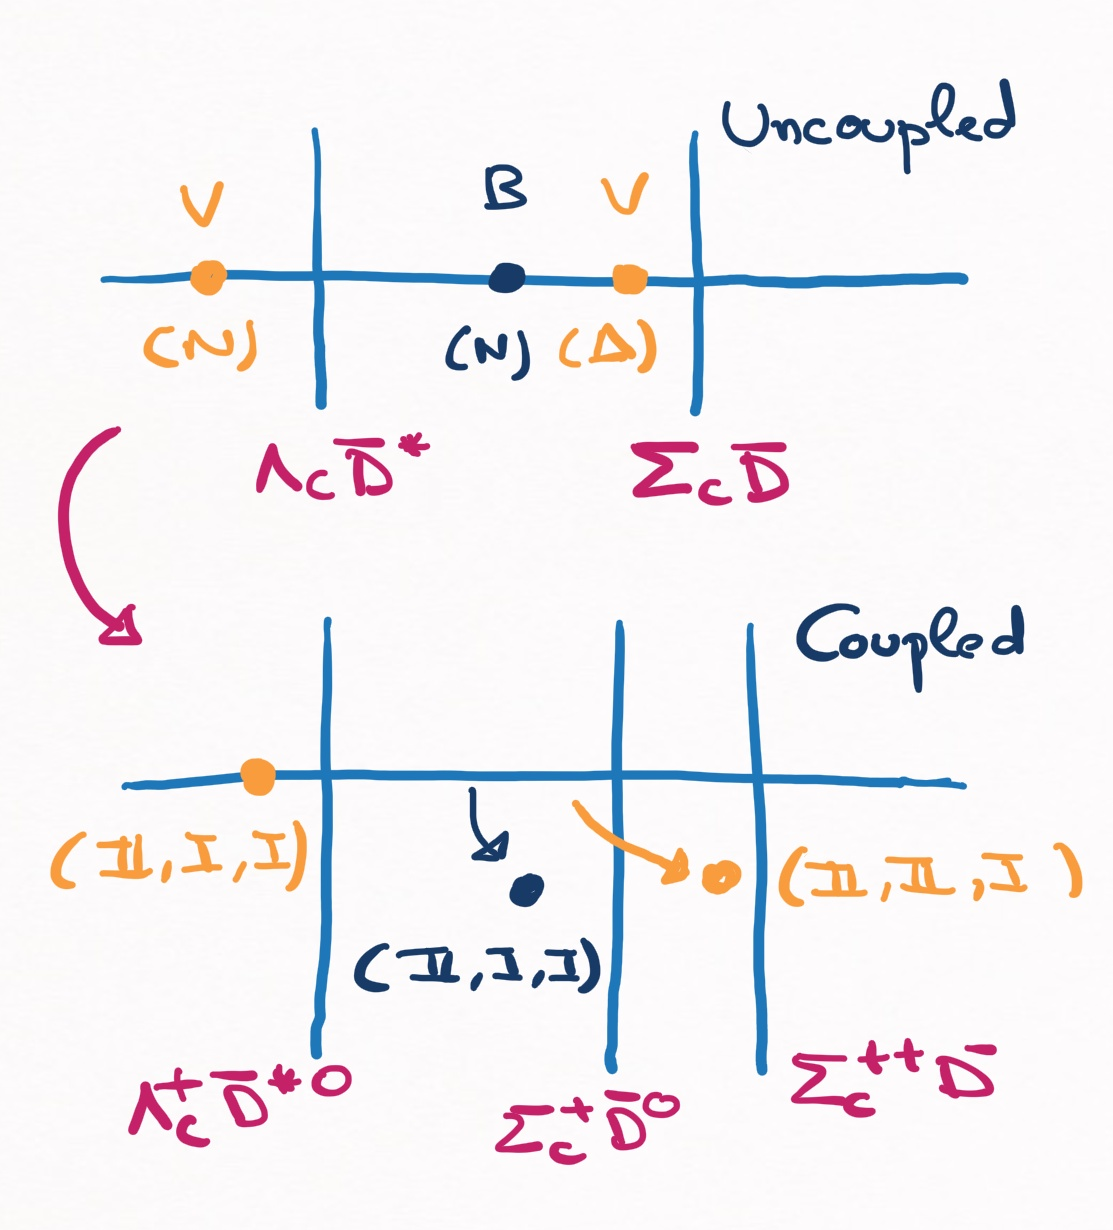
\includegraphics[height=4.5cm]{figures/Pc4337/3-poles.jpeg}
}}
\end{minipage}
\begin{minipage}{0.025\textwidth}
\phantom{O}
\end{minipage}
\begin{minipage}{0.55\textwidth}
  {\small
    \begin{itemize}
    \item Uncoupled + isospin symmetric: \\
      \vspace{0.10cm}
      $\tilde{P}_{\psi}^N$, $P_{\psi}^N$ and $P_{\psi}^{\Delta}$ poles

    \item Coupled (in particle basis): \\
      \vspace{0.10cm}
    $P_{\psi}^N$, $P_{\psi}^{\Delta}$ couplings to $\Sigma_c^+ \bar{D}^0$ and
    $\Sigma_c^{++} {D}^-$ will badly break isospin symmetry!
    \end{itemize}

    \hspace{0.6cm} Calling them $P_{\psi}^N$, $P_{\psi}^{\Delta}$ is just \\
    \vspace{0.01cm} \hspace{0.55cm} a manner of speaking.
    }
\end{minipage}
\end{center}

{\small Note: the $\Lambda_c \bar{D}^*$-$\Sigma_c \bar{D}$ ($I=1/2$)
  non-diagonal interaction is probably important.}


\end{frame}
%---------------------------------------------------------------------- SLIDE -
\begin{frame}
\frametitle{$P_{c}(4337)$ and the $\Lambda_c \bar{D}^*$-$\Sigma_c \bar{D}$ pole structure (II)}

The distributions do not discriminate well the meson-baryon interaction. 

\vspace{0.15cm}
Thus I will only fit the production/decay combined couplings and
consider the following meson-baryon scenarios:

\begin{itemize}
\item[(a)] $\tilde{P}_c^N$, ${P}_c^N$ virtual states, no transition or decuplet potential \\
  {\scriptsize $\tilde{C}_O = -0.343$, $C_E = 0$, $C_O = -0.481$, $C_D = 0$ ($\,{\rm fm}^2)$ \\
    $\tilde{P}_c^N(4276.1)$ virtual,
    ${P}_c^N(4317.5 + i 1.2)$ virtual (II,II,II)}

\item[(b)] $\tilde{P}_c^N$, ${P}_c^{\Delta}$ virtual states, $P_c^N$ bound \\
  {\scriptsize $\tilde{C}_O = -0.372$, $C_E = 0.148$,
    $C_O = -0.802$, $C_D = -0.457$ ($\,{\rm fm}^2$)\\
    $\tilde{P}_c^N(4290.0)$ virtual, ${P}_c^{\Delta}(4327.1 - i 3.5)$ virtual (II,II,II), $P_c^{N}(4310.7 - i 5.2)$ bound}

\item[(c)] ${P}_c^{\Delta}$ bound state, potential rather weak
  in the other channels \\
  {\scriptsize $\tilde{C}_O = +0.138$, $C_E = 0.073$,
    $C_O = -0.165$, $C_D = -0.900$ ($\,{\rm fm}^2$)\\
    ${P}_c^{\Delta}(4302.7 - i 0.0)$ bound (II,I,I), very narrow (components
    widths have not been included: its actual width should be about
    $2\,{\rm MeV}$ give or take), tiny isospin breaking effects.}

\item[(d)] No poles near threshold, weak attraction in all channels \\
    {\scriptsize $\tilde{C}_O = -0.088$, $C_E = -0.129$,
    $C_O = -0.202$, $C_D = -0.207$ ($\,{\rm fm}^2$)}
\end{itemize}

Note: the calculation of the poles assumes stable components!

\end{frame}
%---------------------------------------------------------------------- SLIDE -
\begin{frame}
\frametitle{$P_{c}(4337)$ and the $\Lambda_c \bar{D}^*$-$\Sigma_c \bar{D}$ pole structure (III)}

Interpretation of the previous scenarios:
\begin{itemize}
\item[(a)] Partly similar to JPAC analysis: $P_c(4312)$ as a near-threshold
  virtual state (but adds $\tilde{P}_c$ to the mix).

\item[(b)] Business as usual: $P_c(4312)$ a bound state, while the interaction
  in the other channels is moderately to strongly attractive but not enough
  as to generate new bound states.

\item[(c)] Exotic scenario, but probably incompatible with what is expected
  in most theoretical models.

\item[(d)] Boring scenario: the interaction is rather weak, but still generating
  near-threshold enhancements, cusps, etc. Might be compatible with a few
  theoretical models.
\end{itemize}

\end{frame}
%---------------------------------------------------------------------- SLIDE -
\begin{frame}
\frametitle{$P_{c}(4337)$ and the $\Lambda_c \bar{D}^*$-$\Sigma_c \bar{D}$ pole structure (IVa)}

\only <1>{
  Scenario {\color{blue} (a)}: bin counts

    {\flushleft
      \vspace{0.20cm}
      \colorbox{white}{
        \includegraphics[height=4.0cm]{gnuplot/M12-fit12-T4-bins-a.eps}
        \includegraphics[height=4.0cm]{gnuplot/Mz-fit12-T4-bins-a.eps}
    }}

    \vspace{0.25cm}
    Poisson deviance $D = 17.4$ (with respect to the $M(J/\psi p)$ bin count)
}
  

\only <2>{
    Scenario {\color{blue} (a)}: line shapes (the noise has been removed from the bins)

    {\flushleft
      \vspace{0.20cm}
      \colorbox{white}{
        \includegraphics[height=4.0cm]{gnuplot/M12-fit12-T4-a.eps}
        \includegraphics[height=4.0cm]{gnuplot/Mz-fit12-T4-a.eps}
    }}
    
    \vspace{0.25cm}
    Poisson deviance $D = 17.4$ (with respect to the $M(J/\psi p)$ bin count)
}

\end{frame}
%---------------------------------------------------------------------- SLIDE -
\begin{frame}
\frametitle{$P_{c}(4337)$ and the $\Lambda_c \bar{D}^*$-$\Sigma_c \bar{D}$ pole structure (IVb)}

\only <1>{
  Scenario {\color{blue} (b)}: bin counts

    {\flushleft
      \vspace{0.20cm}
      \colorbox{white}{
        \includegraphics[height=4.0cm]{gnuplot/M12-fit12-T4-bins-b.eps}
        \includegraphics[height=4.0cm]{gnuplot/Mz-fit12-T4-bins-b.eps}
    }}

    \vspace{0.25cm}
    Poisson deviance $D = 19.6$ (with respect to the $M(J/\psi p)$ bin count)
}
  

\only <2>{
    Scenario {\color{blue} (b)}: line shapes (the noise has been removed from the bins)

    {\flushleft
      \vspace{0.20cm}
      \colorbox{white}{
        \includegraphics[height=4.0cm]{gnuplot/M12-fit12-T4-b.eps}
        \includegraphics[height=4.0cm]{gnuplot/Mz-fit12-T4-b.eps}
    }}
    
    \vspace{0.25cm}
    Poisson deviance $D = 19.6$ (with respect to the $M(J/\psi p)$ bin count)
}

\end{frame}
%---------------------------------------------------------------------- SLIDE -
\begin{frame}
\frametitle{$P_{c}(4337)$ and the $\Lambda_c \bar{D}^*$-$\Sigma_c \bar{D}$ pole structure (IVc)}

\only <1>{
  Scenario {\color{blue} (c)}: bin counts

    {\flushleft
      \vspace{0.20cm}
      \colorbox{white}{
        \includegraphics[height=4.0cm]{gnuplot/M12-fit12-T4-bins-c.eps}
        \includegraphics[height=4.0cm]{gnuplot/Mz-fit12-T4-bins-c.eps}
    }}

    \vspace{0.25cm}
    Poisson deviance $D = 16.1$ (with respect to the $M(J/\psi p)$ bin count)
}
  

\only <2>{
    Scenario {\color{blue} (c)}: line shapes (the noise has been removed from the bins)

    {\flushleft
      \vspace{0.20cm}
      \colorbox{white}{
        \includegraphics[height=4.0cm]{gnuplot/M12-fit12-T4-c.eps}
        \includegraphics[height=4.0cm]{gnuplot/Mz-fit12-T4-c.eps}
    }}
    
    \vspace{0.25cm}
    Poisson deviance $D = 16.1$ (with respect to the $M(J/\psi p)$ bin count)
}

\end{frame}
%---------------------------------------------------------------------- SLIDE -
\begin{frame}
\frametitle{$P_{c}(4337)$ and the $\Lambda_c \bar{D}^*$-$\Sigma_c \bar{D}$ pole structure (IVd)}

\only <1>{
  Scenario {\color{blue} (d)}: bin counts

    {\flushleft
      \vspace{0.20cm}
      \colorbox{white}{
        \includegraphics[height=4.0cm]{gnuplot/M12-fit12-T4-bins-d.eps}
        \includegraphics[height=4.0cm]{gnuplot/Mz-fit12-T4-bins-d.eps}
    }}

    \vspace{0.25cm}
    Poisson deviance $D = 16.8$ (with respect to the $M(J/\psi p)$ bin count)
}
  

\only <2>{
    Scenario {\color{blue} (d)}: line shapes (the noise has been removed from the bins)

    {\flushleft
      \vspace{0.20cm}
      \colorbox{white}{
        \includegraphics[height=4.0cm]{gnuplot/M12-fit12-T4-d.eps}
        \includegraphics[height=4.0cm]{gnuplot/Mz-fit12-T4-d.eps}
    }}
    
    \vspace{0.25cm}
    Poisson deviance $D = 16.8$ (with respect to the $M(J/\psi p)$ bin count)
}

\end{frame}
%---------------------------------------------------------------------- SLIDE -
\begin{frame}
  \frametitle{$B^0 \to J/\Psi p \bar{p}$ and the $\Lambda_c \bar{D}$ and
    $\Lambda_c \bar{D}^*$ systems}

  LHCb 2021: $B^0 \to J/\Psi p \bar{p}$ observed too,
  but no mention of the number of events:
  less statistics than for $B_s^0$ ($797 \pm 31)$

  \vspace{0.35cm}
  The decay amplitudes (if meson-baryon loops) are analogous

  \colorbox{white}{
    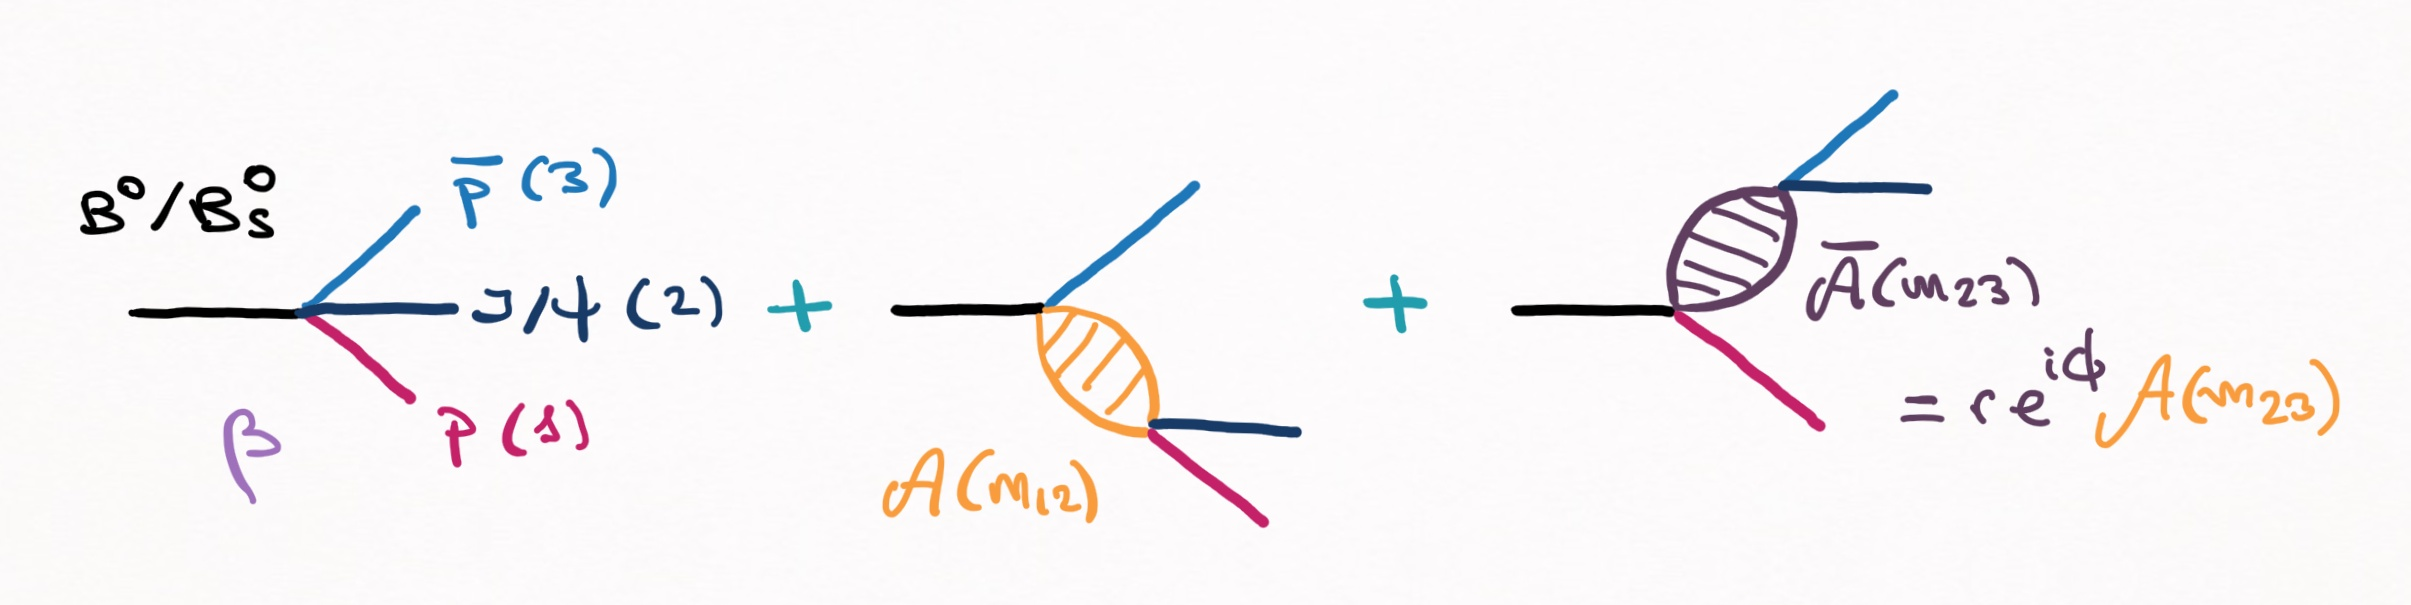
\includegraphics[height=2.00cm]{figures/Pc4337/diagrams-B0-decay.jpeg}
}

  but $B^0$ covers $M(J/\Psi p)$ from $4035$ to $4341\,{\rm MeV}$:
  \begin{itemize}
  \item $\Sigma_c \bar{D}$ poles still visible (though reduced phase space)
  \item $\Lambda_c \bar{D}$ and $\Lambda_c \bar{D}^*$ virtual states might
    be visible \\
    (provided high enough number of events)
  \end{itemize}

  {\color{blue} Very much complementary to $B_s^0 \to J/\psi p \bar{p}$}

  \vspace{0.25cm}

  Basically, {\color{blue} \bf it relies on the same amplitudes already
    calculated here!}
\end{frame}
%---------------------------------------------------------------------- SLIDE -
\begin{frame}
\frametitle{The End}


\begin{center}
  {\Large That's all for the moment.}
\end{center}

\vspace{1.0cm}

\begin{center}
  {This tutorial will be updated as the code base is extended.}
\end{center}

\end{frame}

\end{document}
